%%%%%%%%%%%%%%%%%%%%%%%%%%%%%%%%%%%%%%%%%%%%%%%%%%%%%%%%%%%%%%%%%%%
% Method
% Team:
% Union
% Members: 
% Bernie Huang, Jim Lan, Hoang Tan, Kenny Hsu, Rahul Aditya, Tan Phat, Wei
% Relative files:
% Method_Union.tex
% Note:    
% Do not compile this file compile Main.tex to get the pdf file instead.
%%%%%%%%%%%%%%%%%%%%%%%%%%%%%%%%%%%%%%%%%%%%%%%%%%%%%%%%%%%%%%%%%%%
\subsection{Method} %Please change "Method" to your goal. 
\textit{\footnotesize Author:Bernie Huan, Jim Lan, Hoang Tan, Kenny Hsu, Rahul Aditya, Tan Phat, Wei.}\\

As mentioned in the background, our team used natural language processing in order to generate metadata. 
The scope of metadata processing is about producing at least three types of metadata including author name, title and abstract.


\subsubsection{Title extraction}

We chose python to be the program to catch the title and other metadata.
First step, we import some necessary packages and functions as following:

\begin{enumerate}
	
	\item re: Regular expression package is a useful package which could be applied to the string comparison.
	\item os: This function can connect the python to operating system, so that we can call the path of the files and folders.
	\item nltk: A natural language toolkit.	We use the corpus plaintext function to build the txt file in a folder as corpus.
	\item string:The string package includes a lot of classes such as lowercase, uppercase,punctuation,digits or whitespace...etc.
	
\end{enumerate}  

To begin, all PDF files are converted into txt file with which we want to deal with.
The path is set and the files are stored in a specific folder.
Then, regular expression in python can help capturing the first sentence in the txt files, which have been converted and stored in specific folder in previous step.


\subsubsection{Author extraction}

In this part, we use the existing python packages to achieve our goal.

Also we combine the key word comparison technique to finish this task.
The following step is below:

\begin{enumerate}
	
	\item Section Separation: As we separate the abstract part from the full text, we extract the text above the 
	abstract section and rename as top section. 
	This section contains title, author and email ,etc.
	\item Tokenization: After accessing the top section, we separate the text into each single word. 

	Then we label the words and store within the new list. 
	Eventually, we write the information within the xml file. 
	
\end{enumerate}

The above steps is also available to extracting the location and organization,etc 
when needed. 
The file mainly functioning for this task is Extract\_Authors.py.

As we test the result, our program has been able to extract authors' name.

\subsubsection{Abstract extraction}

Developing from previous theory mentioned in the background section, 
we use the python to catch the abstract.


After being able to read the txt file on every line, 
the python will detect the content of the abstract.
In order to do so, we strip the text between "abstract" label and "introduction" label.	


Abstract-database:including the condition

\begin{enumerate}
	
	\item Capital         "ABSTRACT".
	\item Lower case      "abstract".
	\item In the sentence "Abstract—Word sense ...".
	\item And so on...
	
\end{enumerate}

In the process building "abstract database", we are aware of different papers may have different form of structures 
and writing style, we search through numbers of articles from different journals.

Table below are the results of the search.

%\begin{center}
%\includegraphics[width=\columnwidth]{Table for method Union}.\\
%\includegraphics[width=\columnwidth]{Table 2 for method Union}.\\
%\caption{Result of finding all forms of "abstract", "introduction" written by different authors}
%\end{center}


abstract-database-stop:including the following conditions

\begin{enumerate}
	
	\item The blank line.
	\item Specific words in the beginning "Keywords".
	\item And so on.
	
\end{enumerate}

The intended output are sentences extracted to the txt file.


\subsubsection{References URL extraction}

References URL extraction is very easy and straightforward.

The procedures are below:

\begin{enumerate}
	
	\item First of all, a PDFx package is imported to python.

	
\end{enumerate}

This method can also detects URL,arxiv and doi references.  
Plus,by using this method, we also can easily extract the title, page number and creation date. 


\subsubsection{Search sentences}

The search sentence part is related to the search engine.
After extracting the necessary information, we have to find a way to search these data.
The procefure is following:
\begin{itemize}
	
	%\begin{center}
	%	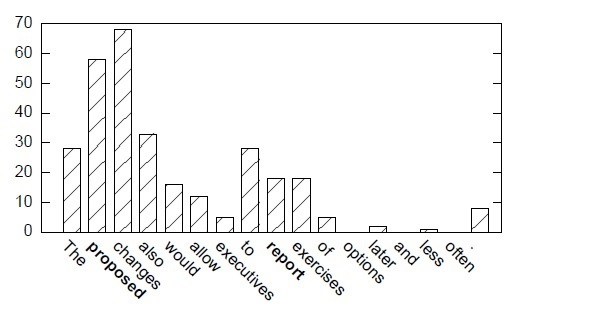
\includegraphics[width=0.8\columnwidth]{Union_Background_Chart_2}
	%\end{center}
	\item First, The PDF is converted to the txt file.(Make the program to read the file name much easier)

	\item Sixth, show the results.
	
\end{itemize}
\subsubsection{API}
We also attempt to produce an semi-automatic interface that help users to inquire certain information from our database. 

said when we still have enough time.
\subsection{Result and discussion}

\newpage % Ends the current page and causes all figures and tables to be printed